\documentclass[conference]{IEEEtran}
\IEEEoverridecommandlockouts\usepackage{cite}
\usepackage{amsmath,amssymb,amsfonts}
\usepackage{algorithmic}
\usepackage{graphicx}
\usepackage{textcomp}
\usepackage{xcolor}
\usepackage{array}
\usepackage{enumitem}
\usepackage{siunitx}
\usepackage[spanish]{babel}
\usepackage{multirow}
\usepackage{float}
\usepackage{booktabs}
\usepackage[hidelinks]{hyperref}
\usepackage{hhline}
\usepackage[left=2cm,right=2cm,top=2cm,bottom=2cm]{geometry}
\usepackage{listings}


\def\BibTeX{{\rm B\kern-.05em{\sc i\kern-.025em b}\kern-.08em
    T\kern-.1667em\lower.7ex\hbox{E}\kern-.125emX}}
    
\begin{document}

\title{Microcontroladores: Laboratorio 1\\
{\footnotesize \textsuperscript{}
}
\thanks{}
}

\author{\IEEEauthorblockN{1\textsuperscript{st} Hector Pereira}
\IEEEauthorblockA{\textit{Ingeniería en Mecatrónica} \\
\textit{Universidad Tecnológica (UTEC)}\\
Fray Bentos, Uruguay \\
hector.pereira@estudiantes.utec.edu.uy}
\and
\IEEEauthorblockN{2\textsuperscript{nd} Mateo Lecuna }
\IEEEauthorblockA{\textit{Ingeniería en Mecatrónica} \\
\textit{Universidad Tecnológica (UTEC)}\\
Fray Bentos, Uruguay \\
mateo.lecuna@estudiantes.utec.edu.uy}
\and
\IEEEauthorblockN{3\textsuperscript{rd} Mateo Sanchez }
\IEEEauthorblockA{\textit{Ingeniería en Mecatrónica} \\
\textit{Universidad Tecnológica (UTEC)}\\
Maldonado, Uruguay \\
mateo.sanchez@estudiantes.utec.edu.uy}
}
\maketitle


\begin{abstract}
Se presenta el diseño e implementación de cuatro subsistemas sobre el microcontrolador ATmega328P: una matriz de LEDs 8x8, un plotter cartesiano, un conversor digital-analógico y una punzonadora con cinta. Cada módulo ejercita competencias clave de sistemas embebidos: multiplexado de filas/columnas y manejo de temporizadores, interpretación de comandos y generación de trayectorias, síntesis y verificación de señales, y control secuencial por máquina de estados con disparo desde USART y pulsadores. 
Se validó el funcionamiento estable de los módulos, con latencia de comunicación adecuada y formas de onda coherentes con lo esperado. Como líneas de mejora se identificaron el uso de PWM para control fino de brillo y velocidad, perfiles de movimiento para el plotter e integración de sensores en la lógica de estados de la punzonadora.
\end{abstract}

\textit{Keywords: ATmega328P, AVR, sistemas embebidos, matriz de LEDs, multiplexado, temporizadores, interrupciones, USART, plotter cartesiano, trayectorias, conversor digital-analógico, PWM, máquina de estados.}

\section{Introducción}

\subsection{Plotter}

\subsection{Sistema de Control de Temperatura}

\subsection{Control de Motor }

\subsection{Matriz RGB con Joystick}

\subsection{Cerradura RFID}

\section{Marco Teórico}

\subsection{Piano}
El piano electrónico se basa en el microcontrolador ATmega328P, encargado de leer las entradas digitales provenientes de pulsadores y generar las notas musicales correspondientes a través de un buzzer piezoeléctrico. Para la síntesis de sonido, se hace uso de señales de modulación por ancho de pulso (PWM), configuradas mediante los temporizadores internos del microcontrolador, permitiendo así obtener frecuencias precisas asociadas a cada nota musical.

El sistema implementa un conjunto de 12 pulsadores, cada uno asignado a una nota de la escala cromática (Do, Do\#, Re, Re\#, Mi, Fa, Fa\#, Sol, Sol\#, La, La\#, Si). Además, se integran dos pulsadores adicionales para modificar la octava activa, lo que amplía la capacidad tonal del instrumento sin aumentar significativamente el número de entradas físicas.

El buzzer piezoeléctrico utilizado actúa como transductor electroacústico, recibiendo la señal PWM generada por el ATmega328P y transformándola en vibraciones audibles. El uso de resistencias pull-up internas en los pines de entrada digital simplifica el cableado, evitando la necesidad de resistencias externas para los pulsadores.

Por otra parte, la inclusión de la comunicación serial mediante UART (Universal Asynchronous Receiver-Transmitter) permite la selección de canciones predefinidas almacenadas en memoria. De esta forma, el sistema no solo funciona como piano manual, sino también como reproductor automático de melodías programadas.

Se implemento de la octava 4 a la 7, por que si se implementaba una ocatava menos, el buzzer ya no podía emitir un sonido distinguible, y emitía siempre el mismo sonido, osea, estaba en su limite, y si se implementaba una octava más por arriba de la 7, el buzzer no podía emitir el sonido, por que también estaba fuera de su rango.

En la sección de anexos, dentro de tablas complementarias~\ref{tab:notas_piano}, se detalla la correspondencia entre las notas musicales y sus frecuencias asociadas, así como el índice utilizado en el arreglo de notas dentro del código fuente del proyecto.

\subsection{Cerradura elctrónica}



\section{Metodología}

\subsection{Plotter}

\subsection{Sistema de Control de Temperatura}

\subsection{Control de Motor }

\subsection{Matriz RGB con Joystick}

\subsection{Cerradura RFID}

\section{Resultados}
\subsection{Conversor digital-análogo}

\begin{verbatim}
RESET:
    ; Apuntar Z al inicio de la LUT
    ldi ZH, HIGH(LUT_START<<1)
    ldi ZL, LOW(LUT_START<<1)

	; Apuntar Y al final de la LUT
	ldi YH, HIGH(LUT_END<<1)
	ldi YL, LOW(LUT_END<<1)
\end{verbatim}

\begin{verbatim}
MAIN_LOOP:
    ; Leer siguiente valor de la LUT
    ; y avanzar puntero
    lpm r16, Z+
    out PORTD, r16
    rcall delay

    cp  ZL, YL
    cpc ZH, YH
    ; Si no es el fin, seguir
    brne MAIN_LOOP

    ; Volver al inicio de la tabla
    ldi ZH, HIGH(LUT_START<<1)
    ldi ZL, LOW(LUT_START<<1)
    rjmp MAIN_LOOP
\end{verbatim}

\begin{figure}[H]
  \centering
  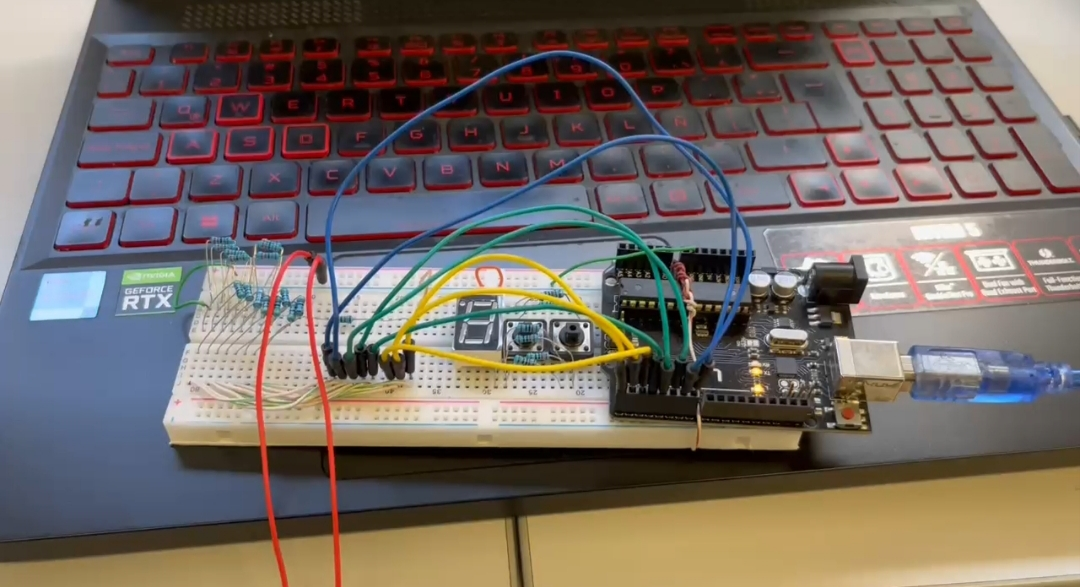
\includegraphics[width=\linewidth]{./Anexos/Resultados/DAC/Circuito.jpg}
  \caption{Circuito final para conversor digital-análogo. Fuente: \cite{LabDrive}.}
  \label{fig:conversor_circuito}
\end{figure}

\begin{figure}[H]
  \centering
  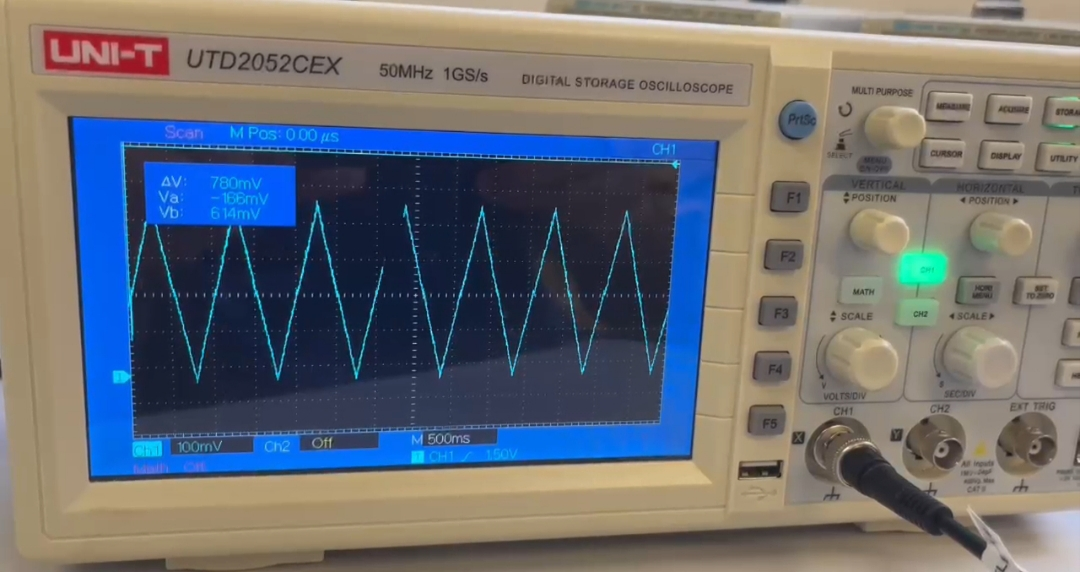
\includegraphics[width=\linewidth]{./Anexos/Resultados/DAC/Ocsiloscopio.jpg}
  \caption{visualización de señal en osciloscopio. Fuente: \cite{LabDrive}.}
  \label{fig:conversor_osciloscopio}
\end{figure}

\subsection{Matriz}

\subsubsection{Mapeado de puertos y pines}
Se mapean los puertos y pines individuales del mismo modo al que se puede apreciar en el anexo \ref{anexo:Look_Up_Table}.

\subsubsection{Encendido de un solo LED}
\begin{verbatim}
ldi ZH, high(ROW_PORTS<<1) 
ldi ZL, low(ROW_PORTS<<1)
add ZL, row adc ZH, r1  
lpm r16, Z ; r16 = row port adress
        
ldi ZH, high(ROW_MASKS<<1) 
ldi ZL, low(ROW_MASKS<<1)
add ZL, row adc ZH, r1
lpm r17, Z ; r18 = row pin mask

; Encender fila
clr ZH mov ZL, r16 
mov r16, r17
rcall CLEAR_BIT

ldi ZH, high(COL_PORTS<<1) 
ldi ZL, low(COL_PORTS<<1)  
add ZL, col adc ZH, r1  
lpm r16, Z ; r16 = column port adress

ldi ZH, high(COL_MASKS<<1) 
ldi ZL, low(COL_MASKS<<1)  
add ZL, col adc ZH, r1  
lpm r17, Z ; r17 = column pin mask

; Encender columna
clr ZH mov ZL, r16 
mov r16, r17
rcall SET_BIT
\end{verbatim}

\subsubsection{Multiplexado y dibujo de cuadros}
\begin{verbatim}
ldi row, 0 RENDER_FRAME_ROW_LOOP:  
ldi r16, 0b00000001 ; Frame mask
lpm r17, Z+

ldi col, 0 RENDER_FRAME_COL_LOOP:
    rcall CLEAR_MATRIX

    push r16
    and r16, r17

    cpi r16, 0 
    breq RENDER_FRAME_SKIP_LED

    rcall TURN_LED
    rcall TEST_DELAY

    RENDER_FRAME_SKIP_LED:
    pop r16
    lsl r16
inc col cpi col, 8 
brlo RENDER_FRAME_COL_LOOP 

inc row cpi row, 8 
brlo RENDER_FRAME_ROW_LOOP
\end{verbatim}

Manejo de cambio de estados utilizando USART para mostrar las diferentes imágenes en la matriz

\begin{verbatim}
USART_RX_ISR:	
    lds r16, UDR0

    ; Apagar pantalla
    cpi r16, '0' 
    breq USART_RX_ISR_CASE_0 

    ; Texto desplazante
    cpi r16, '1' 
    breq USART_RX_ISR_CASE_1 

    ; ...

USART_RX_ISR_CASE_0:
    rcall SET_ANIMATION_START
    ; Disable timer interrupts
    ldi r16, 0b0 sts TIMSK2, r16 
    ; Change state
    ldi r16, 0 mov current_state, r16   
    rjmp USART_RX_ISR_END

USART_RX_ISR_CASE_1:
    rcall SET_ANIMATION_START
    ; Change state
    ldi r16, 1 mov current_state, r16   
    ; Enable timer interrupts
    ldi r16, 0b1 sts TIMSK2, r16 
    rjmp USART_RX_ISR_END

    ; ...
\end{verbatim}

Aparte del manejo del cambio de estado, se implementó una máquina de estados, como la que se puede encontrar en el anexo \ref{anexo:Maquina_de_Estados}.

\begin{verbatim}
MAIN:
    rcall STATE_MACHINE
    rjmp MAIN
\end{verbatim}

Circuito final realizado:

\begin{figure}[H]
  \centering
  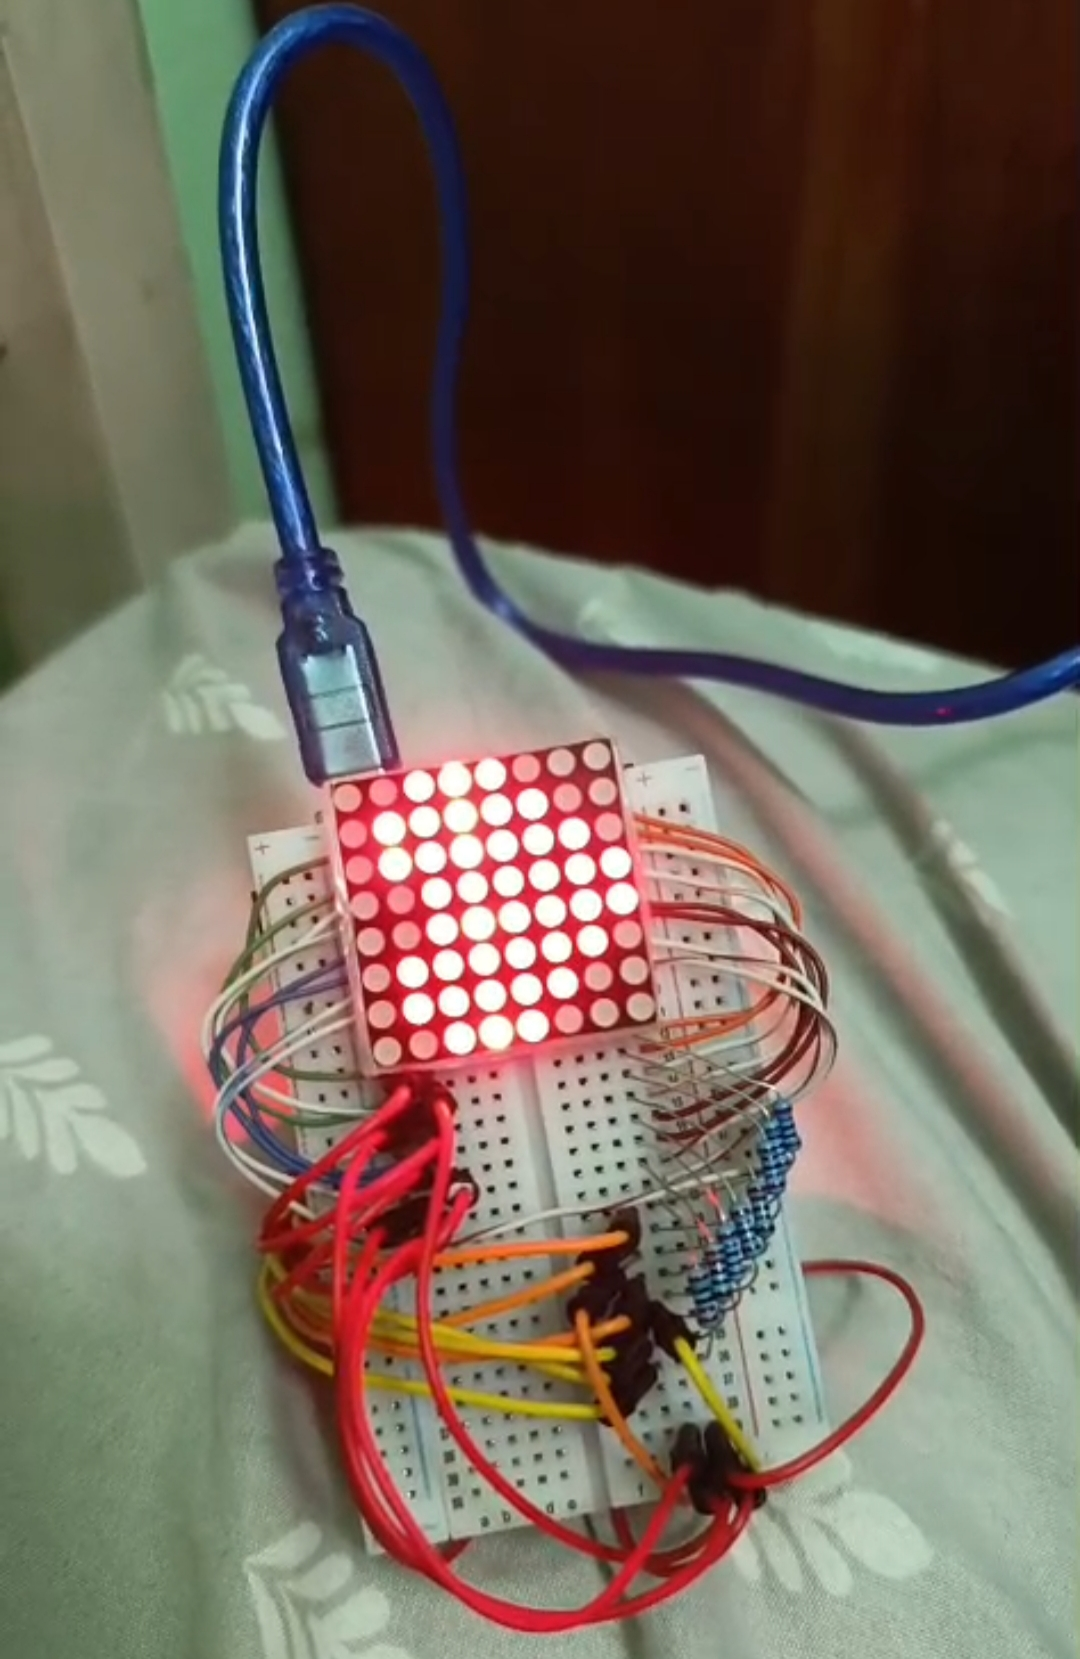
\includegraphics[width=0.7\linewidth]{./Anexos/Resultados/Matriz/Circuito.jpg}
  \caption{Circuito final para Matriz de LEDs. Fuente: \cite{LabDrive}.}
  \label{fig:circuito_matriz}
\end{figure}


\section{Punzonadora}

\subsubsection{Configuración de temporizador variable}
\begin{verbatim}
.macro ENABLE_TIMER_1
; @0 Timer seconds
push r16
mov timer1_ovf_counter, @0
ldi r16, 0b101		 sts TCCR1B, r16
ldi r16, HIGH(49911) sts TCNT1H, r16
ldi r16, LOW(49911)	 sts TCNT1L, r16 
ldi r16, (1<<TOV1)   out TIFR1,  r16 
ldi r16, (1<<TOIE1)  sts TIMSK1, r16 
pop r16
.endmacro
\end{verbatim}


\subsubsection{Manejo de estados}

Control de estados general:
\begin{verbatim}
STATE_MACHINE:
cpi state, 0 breq STATE_MACHINE_STOP
cpi state, 1 breq STATE_MACHINE_ADVANCE
cpi state, 2 breq STATE_MACHINE_WAIT_1
cpi state, 3 breq STATE_MACHINE_PUNCH
cpi state, 4 breq STATE_MACHINE_WAIT_2
cpi state, 5 breq STATE_MACHINE_EXTRACT
rjmp STATE_MACHINE_END
\end{verbatim}

Control de estados individual, cada caso tiene un manejo de tiempos específico dictado por el diagrama de estados mostrado con anterioridad.
\begin{verbatim}
STATE_MACHINE_STOP:
cpi load, 0 breq STOP_LOAD_0
cpi load, 1 breq STOP_LOAD_1
cpi load, 2 breq STOP_LOAD_2
rjmp STATE_MACHINE_STOP_SKIP
\end{verbatim}

\subsubsection{Botones, LEDs,  y debouncing}
Interrupción se descativa sola. Se vuelve a habilitar cuando la máquina de estados llega al final del recorrido:

\begin{verbatim}
INT0_ISR:
    push r16
    in r16, SREG
    push r16 

    DISABLE_BUTTONS
    DISABLE_RX

    ldi state, 1
    ldi r16, 1 
    sts event_pending, r16

    pop r16
    out SREG, r16
    pop r16 
    reti
\end{verbatim}

Temporizador de deboucing para botones de cambio de carga. Timer 2 configurado para un overflow de aproximadamente 1 segundo (usando contador de overflow externo):

\begin{verbatim}
    T2_OVF_ISR:
	push r16 
    in r16, SREG 
	push r16 
	
	inc timer2_ovf_counter
	
	ldi r16, _TIMER2_OVF_COUNT 
    cp r16, timer2_ovf_counter 
    brsh T2_OVF_ISR_END 
    
	DISABLE_TIMER_2
	ENABLE_BUTTONS
	clr timer2_ovf_counter
    
    T2_OVF_ISR_END:
		pop r16
		out SREG, r16
		pop r16	
		reti

\end{verbatim}

\subsubsection{USART}
Identico para los otros casos, se configura un menú que es enviado en el RESET del programa para ser mostrado al inicio, y una serie de condicionales determinan el comportamiento del sistema dependiendo del comando que recibe. En este caso: 1, 2, y 3 para seleccionar el tipo de carga. Y A para iniciar la secuencia del programa.


\begin{figure}[H]
  \centering
  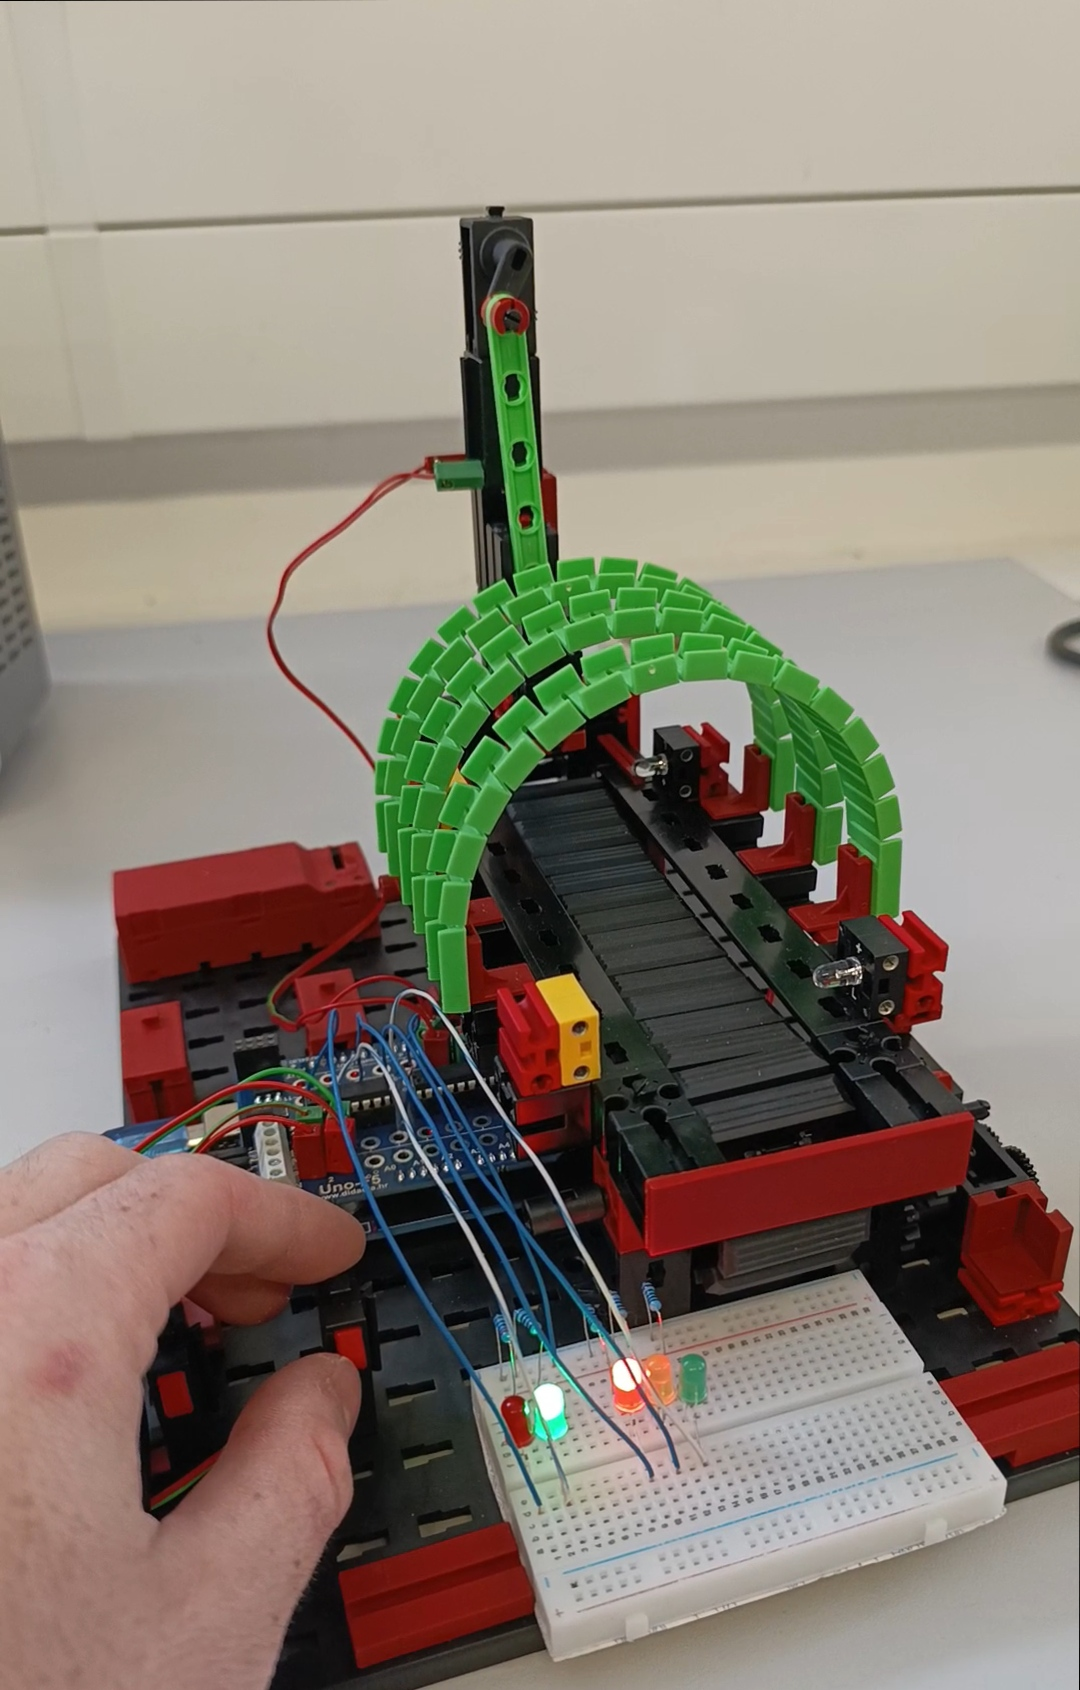
\includegraphics[width=0.7\linewidth]{./Anexos/Resultados/Punzonadora/Circuito.jpg}
  \caption{Ensamblado final de punzonadora. Fuente: \cite{LabDrive}.}
  \label{fig:punzonadora_circuito}
\end{figure}


\subsection{Plotter}

\subsubsection{Mapeo de comandos}
\begin{verbatim}
.equ SOLENOID_DOWN =	0b00000100
.equ SOLENOID_UP =		0b00001000
.equ DOWN =				0b00010000
.equ UP =				0b00100000
.equ RIGHT =			0b01000000
.equ LEFT =				0b10000000
.equ STOP =				0b00000000
\end{verbatim}
\subsubsection{Interprete de secuencias}
\begin{verbatim}
DRAW:
    mov ZL, r16 mov ZH, r17
    DRAW_LOOP:
    lpm r18, Z+ ; Time
    lpm r19, Z+ ; Instruction

    out PORTD, r19 ; Send instruction

    cpi r19, STOP
    breq DRAW_END ; Stop drawing

    DRAW_TIMER_LOOP: ; Timer
    rcall S1
    dec r18 brne DRAW_TIMER_LOOP 

    rjmp DRAW_LOOP ; Next instruction

    DRAW_END:
    ret
\end{verbatim}
Nota: se encontró que para temporizadores con valores menores a 1ms no permitían el movimiento adecuado de los motores, por lo cual se decidió limitar la resolución con un temporizador de 1500 $\mu S$
El siguiente ejemplo es de un programa hecho para el interprete creado para el plotter:
\begin{verbatim}
TRIANGLE_DATA:
    .db 5, SOLENOID_DOWN	
    .db 20, SOLENOID_DOWN + RIGHT			
    .db 10, SOLENOID_DOWN + UP + LEFT		
    .db 10, SOLENOID_DOWN + DOWN + LEFT
    .db 5, SOLENOID_UP		
    .db 5, STOP
\end{verbatim}

\subsubsection{USART}
Ejemplo de caso de interrupción de USART para dibujado de circulo:
\begin{verbatim}
; ...
USART_RX_ISR_CASE_5: ; CIRCLE
    ldi r16, low(CIRCLE_DATA<<1) 
    ldi r17, high(CIRCLE_DATA<<1)
    rcall DRAW
    rjmp USART_RX_ISR_END
\end{verbatim}

\begin{figure}[H]
  \centering
  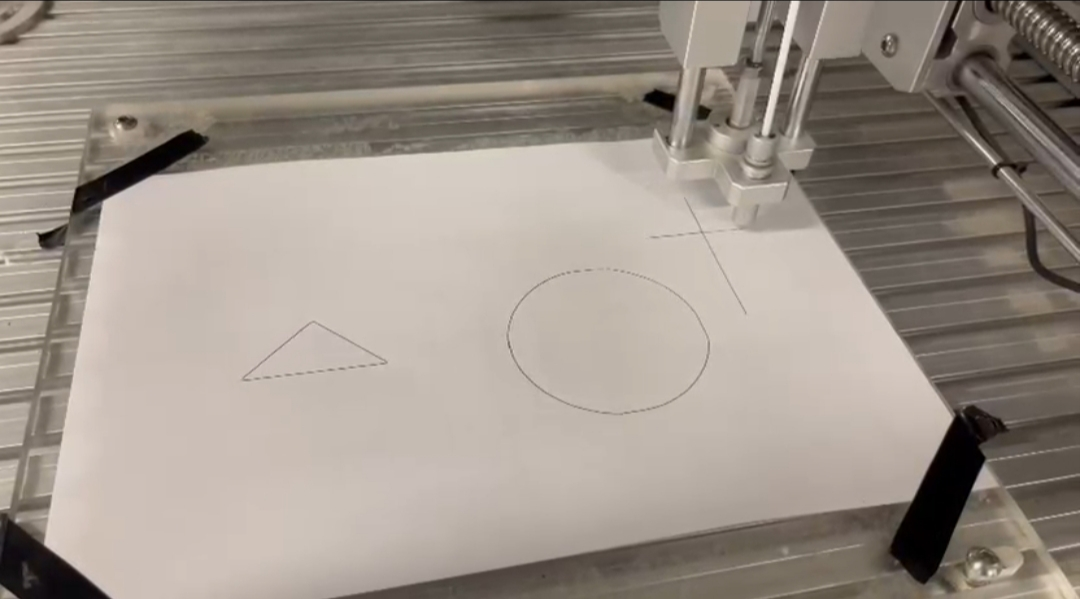
\includegraphics[width=\linewidth]{./Anexos/Resultados/Plotter/Dibujos.jpg}
  \caption{Figuras dibujadas en el plotter. Fuente: \cite{LabDrive}.}
  \label{fig:plotter_figuras}
\end{figure}

\section{Conclusiones}
\subsection{Plotter}

\subsection{Sistema de Control de Temperatura}

\subsection{Control de Motor }

\subsection{Matriz RGB con Joystick}

\subsection{Cerradura RFID}

            
\bibliographystyle{IEEEtran}
\nocite{*}
\bibliography{5_referencias}

\newpage

\section{Anexos}

\subsection{Esquemas de conexión}

\subsubsection{Piano electrónico}

En la Figura~\ref{fig:conexion_piano} se muestra el esquema de conexión del piano electrónico, elaborado en Tinkercad®. 
Se pueden observar las conexiones entre el microcontrolador ATmega328P, los pulsadores, y el buzzer piezoeléctrico pasivo EMX-7T05SP.

\begin{figure}[H]
    \centering
    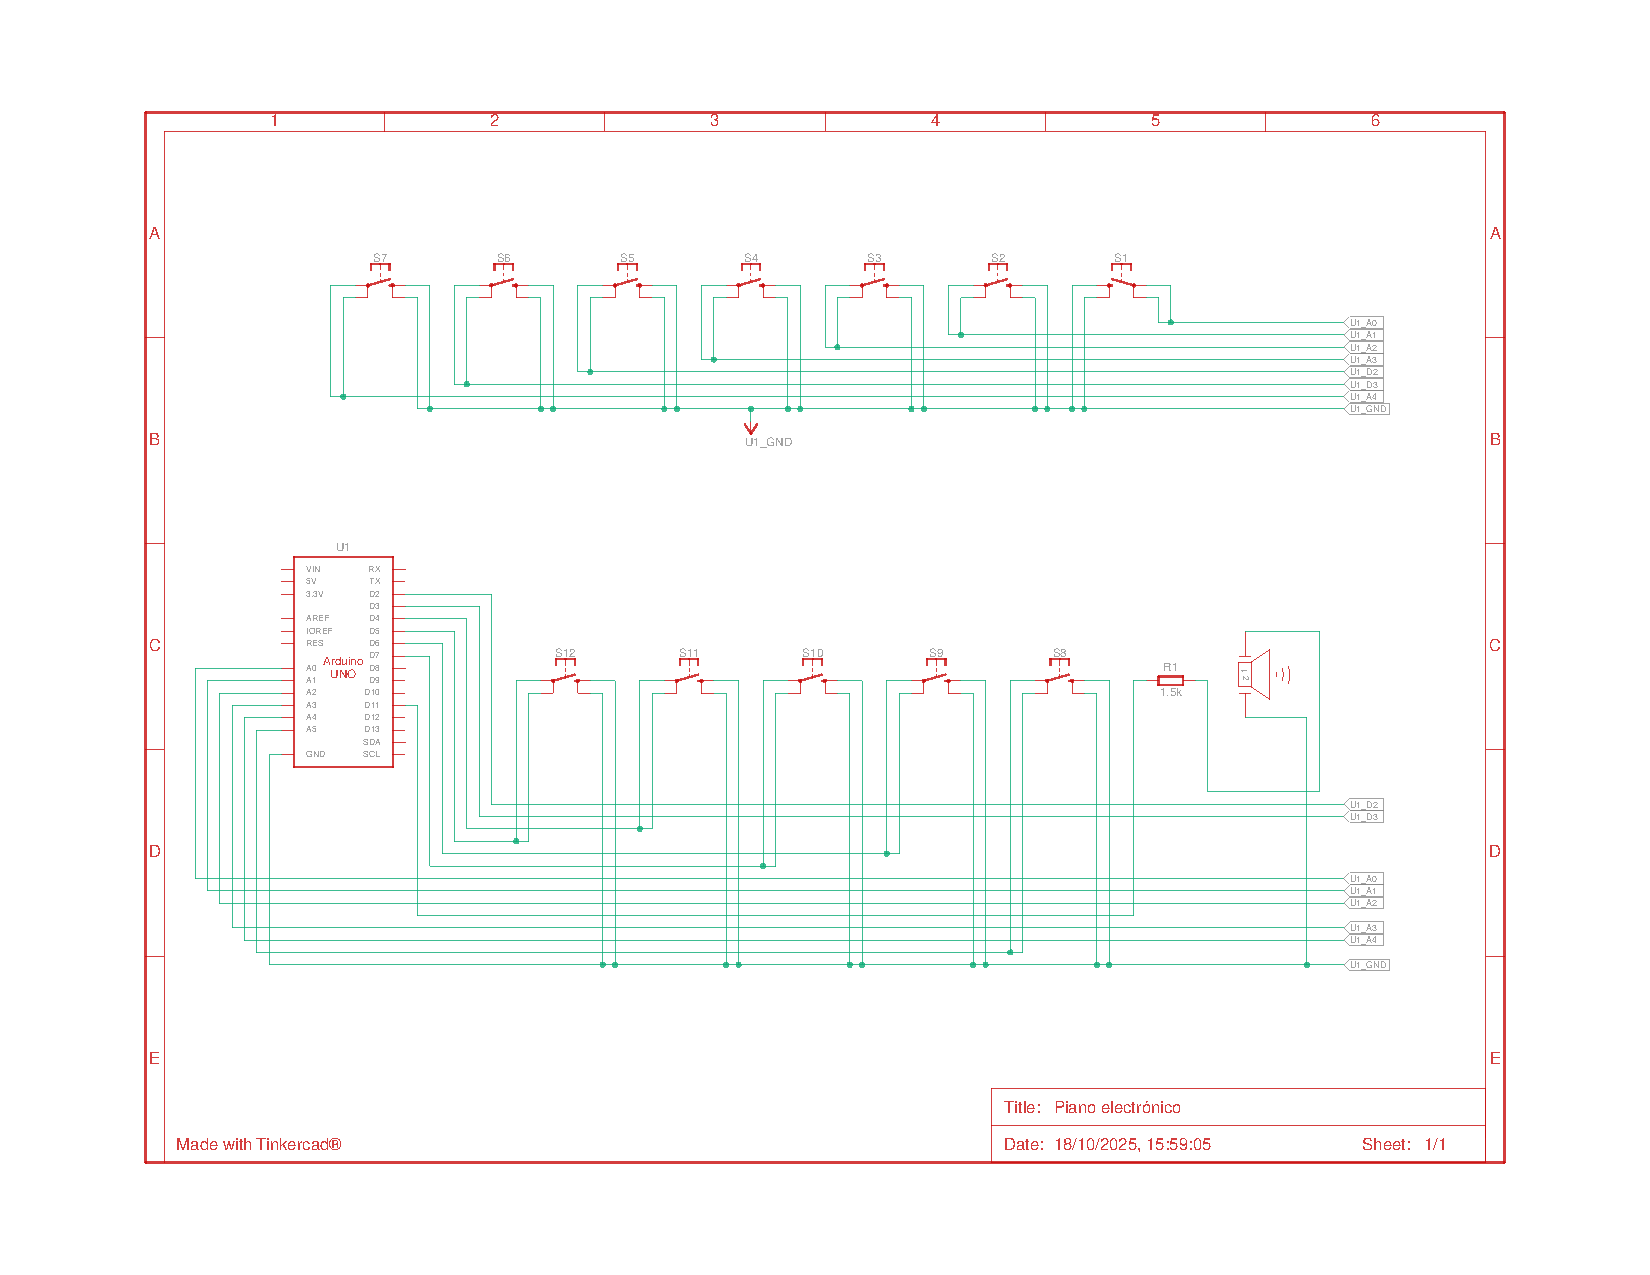
\includegraphics[width=0.5\textwidth]{Anexos/Conexionado_de_piano.pdf}
    \caption{Esquema de conexión del piano electrónico. Elavoración propia en Tinkercad®.}
    \label{fig:conexion_piano}
\end{figure}

\subsubsection{Cerradura electrónica}

En la Figura~\ref{fig:Cerradura_electronica} se presenta el esquema de conexión del sistema de cerradura electrónica. 
El circuito fue diseñado en Tinkercad® y muestra la interconexión entre el microcontrolador ATmega328P, el teclado matricial 4×4, 
la pantalla LCD 16×2 con interfaz I²C, los LEDs indicadores (rojo y verde) y el buzzer de señalización.

\begin{figure}[H]
    \centering
    \includegraphics[width=0.5\textwidth]{Anexos/Cerradura_electrónica.pdf}
    \caption{Esquema de conexión del candado electrónico. Elaboración propia en Tinkercad®.}
    \label{fig:Cerradura_electronica}
\end{figure}


\end{document}